\documentclass[a4paper,12pt]{article}
%For images
\usepackage{graphicx}
 
\addtolength{\oddsidemargin}{-.875in}
\addtolength{\evensidemargin}{-.875in}
\addtolength{\textwidth}{1.75in}
 
\addtolength{\topmargin}{-.875in}
\addtolength{\textheight}{1.75in}
 
\begin{document}
\begin{enumerate}
    \item \begin{enumerate}
        \item Med produktregeln blir derivatan
        $$x'cos(x)+x(cos(x))'=cos(x)-xsin(x)$$

        \item Med produktregeln blir derivatan
        $$\frac{e^x}{x}-\frac{e^x}{x^2}$$
    \end{enumerate}

    \item \begin{enumerate}
        \item Derivatan är 

        \item $$y'(x)=-\frac{4}{x^2}+\frac{1}{x}$$
        Så 
        $$y'(2)=-\frac{4}{4}+\frac{1}{2}=-0.5$$

        Vilket kan verifieras med en bild

        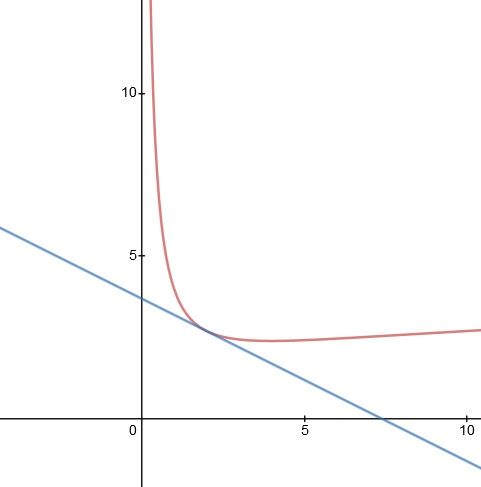
\includegraphics[scale=0.5]{Figur 1.jpg}
    \end{enumerate}

    \item
    Derivatan blir
    $$\frac{10}{x}-2x+8$$

    Som illustreras som röd medans den svarta är orginalekvationen.
    
    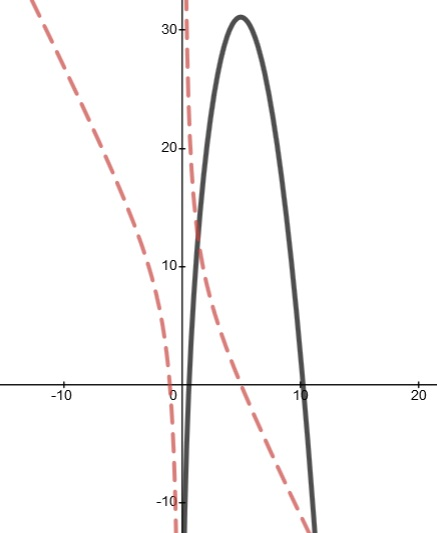
\includegraphics[scale=0.6]{Figur 2.jpg}
    
    Extrempunkterna hamnar där derivatan är noll
    $$\frac{10}{x}-2x+8=0$$
    Skriver om den till en andragradsekvation
    $$10-2x^2=-8x\Rightarrow x^2-4x-5=0\Rightarrow (x-5)(x+1)=0$$
    Extrempunkterna sker då vid 5 och -1.
    Man kan se vid dom olika omskrivningarna av derivatan
    så behåller möter dom fortfarande varandra på x-axeln

    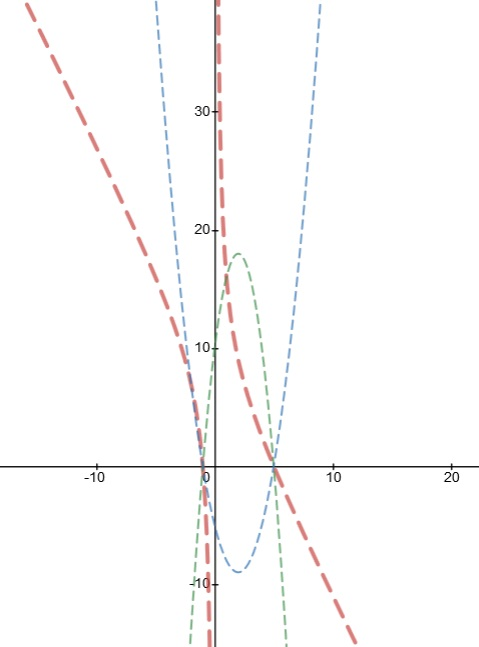
\includegraphics[scale=0.6]{Figur 3.jpg}

    Men eftersom att den orginella ekvationen inehåller
    $10ln(x)$ så är den odefinierad för reella variabler.
    Då lär jag svara att det finns en extrempunkt vid x=5

    Tar man andraderivatan $-\frac{10}{x^2}-2$ vid x=5 får man att 
    andraderivatan är negativ, vilket innebär att det är en maximipunkt.   
    Detta kan man se i figur 2. 

    \item 
\end{enumerate}
\end{document}